\section{VERIFICATION OF REQUIREMENTS}




%\begin{slshape}
%\color{blue}
%
%We have to know that we designed what we were required to design by this document.  This process is called `verification' and it answers the fundamental question: ``Did we build what we said we would build?".  We verify requirements by testing to see if the requirements are met.  Design teams must test every requirement in order to prove that the requirement is met.  Testing each requirement means that each requirement must cast in some quantifiable way.  In this section you specify how you will test each requirement to show that it has been met.
%\bigskip
%
%Don't worry!  It is not as bad as it sounds.  Sometimes (not always!) you can verify or test a requirement simply by looking at the completed system to make sure some required thing is present. 
%\bigskip
%
%Testing often `takes it on the chin' in terms of project schedule.  Since integrated system testing typically occurs near the end of a project, the time for testing is compressed against the deadline.  People start short-cutting tests to stay on schedule.  Sometimes you may get away with it but it is never a good idea either technically or ethically.  Epic failures have occurred because of truncated testing.  One such failure occurred during the testing of the Hubble Space Telescope.  The following is an excerpt from the the official report detailing the failure.
%
%\begin{quote}
%Reliance on a single test method was a process which was clearly
%vulnerable to simple error. Such errors had been seen in other telescope
%programs, yet no independent tests were planned, although some simple tests to
%protect against major error were considered and rejected. During the critical time
%period, there was great concern about cost and schedule, which further inhibited
%consideration of independent tests.\\
%\bigskip
%The Hubble Space Telescope Optical Systems Failure Report-NASA November 1990 
%\end{quote}
%\bigskip
%
%If you are interested the whole report is available at (\url{https://www.ssl.berkeley.edu/~mlampton/AllenReportHST.pdf}).
%\bigskip
%
%The Hubble error wasn't caught until the telescope was deployed in space.  Can you imagine the cost of fixing this problem?  It is not simply a case of bundling you off with your instruments and putting you up in a fancy hotel for a week or two.  Some estimates set the price at about \$1 billion.
%\bigskip
%
%The Dilbert comic strip has a similar, and darkly amusing, view of testing truncation.
%\bigskip  
%
%(\url{http://dilbert.com/strip/2010-08-21})
%\bigskip
%
%(\url{http://dilbert.com/strip/2009-07-01})
%\bigskip
%
%
%
%	
%The key to completing this section is that every requirement has an associated test.  The best practice in this section is to match the sub-paragraph numbers in the previous section to the sub-paragraph numbers in this section, e.g the requirement in 4.3.1.6 is covered by the test described in 5.3.1.6.
%\bigskip
%
%	Possible verification methods include:
%	\bigskip
%	
%	\begin{enumerate}
%		\item Inspection:\\
%
%	Inspection is a method of verification consisting of investigation, 
%	without the use of special laboratory appliances or procedures, to 
%	determine compliance with requirements. Inspection is generally 
%	nondestructive and includes (but is not limited to) visual examination, 
%	manipulation, gauging, and measurement.
%
%		\item Demonstration:\\
%
%	Demonstration is a method of verification that is limited to readily 
%	observable functional operation to determine compliance with 
%	requirements. This method shall not require the use of special equipment 
%	or sophisticated instrumentation.
%	
%		\item Analysis:\\
%
%	Analysis is a method of verification, taking the form of the processing of 
%	accumulated results and conclusions, intended to provide proof that 
%	verification of a requirement has been accomplished. The analytical 
%	results may be based on engineering study, compilation or interpretation 
%	of existing information, similarity to previously verified requirements, 
%	or derived from lower level examinations, tests, demonstrations, or 
%	analyses.
%
%
%		\item Direct Test:
%
%	Test is a method of verification that employs technical means, including (but not 
%	limited to) the evaluation of functional characteristics by use of special equipment
%	or instrumentation, simulation techniques, and the application of established 
%	principles and procedures to determine compliance with requirements.
%			
%	\end{enumerate}		
%	
%\end{slshape}
%
%\subsection{Verify Coverage of Stakeholder Requirements}
%
%\begin{slshape}
%\color{blue}
%The tester verifies that everything that the stakeholders have asked for are covered by one or more requirements.  It is a good idea for the requirements author(s) to perform a similar check at this point.  The tester is likely to do his own analysis or disagree on points in yours, but the exercise itself is valuable. And if you do the analysis you might as well write it down here.   
%\end{slshape}


\subsection{System Overview} 
The Backyard Splash Pad is comprised of four main components: a device controller, a user interface, a mechanical system, and an object-tracking system. 
The device controller receives input from the user interface and uses it to control the mechanical system.
The user interface presents information about the system to the user and accepts input from the user.
The mechanical system controls the flow of water. 
The object-tracking system detects objects near the Splash Pad and reports information to the controller. 
See Figure \ref{fig:functional_diagram_}.

\subsubsection{Functional Diagram}
Test by confirming that each element of the functional diagram is present in the final design. 

\begin{figure}[h]
\centering
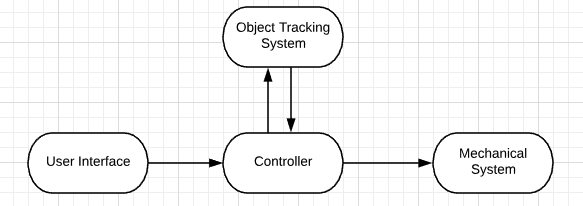
\includegraphics[width=0.9\textwidth]{Functional_Diagram.png}
\caption{\label{fig:functional_diagram_}Functional Diagram.}
\end{figure}

\subsection{Functional Requirements}

\subsubsection{Controller}
%The controller is the part of the system that controls the physical outputs. 

\paragraph{Stream Control}
%The controller shall be able to turn on and off each water stream individually.
Test by observing that each stream turns on and turns off.

\paragraph{Light Control}
%The controller shall be able to turn on and off each light individually.
Test by observing that each light turns on and turns off.

\paragraph{Color Control}
%The controller shall be able to change the color of each light individually.
Test by observing that each light changes color.

\paragraph{Responsive to Object Tracking System} 
%The controller shall be able to turn on a specified nozzle as directed by the Object Tracking System.
Enable the object tracking system. Observe that a water stream turns on due to input from the Object Tracking System.

\paragraph{Programmed Display}
%The controller shall have at least one pre-programmed fountain routine containing light changes and water streams turning on and off.
Use the user interface to run the fountain routine. Observe that lights change and water streams turn on and off.

\subsubsection{User Interface}
%The user interface is the part of the system that accepts input from the user and translates it into commands that the controller can execute. 


\paragraph{User Nozzle Control}
%The user interface shall allow the user to select what nozzle(s) are turned on.
Use the user interface to turn on a water stream. Observe that the water stream turns on.

\paragraph{User Color Control}
%The user interface shall allow the user to select what color the LEDs are.
Use the user interface to change the color of a light. Observe that the color of the light changes. 

\paragraph{User Object Tracking Control}
%The user interface shall allow the user to enable or disable the object tracking system.
Use the user interface to disable the Object Tracking System. Place a basketball-sized object (or larger) near a nozzle. Observe the the splash pad does not react to the presence of the object. 

\subsubsection{Mechanical System}
%The mechanical system is the physical aspect of the system. The mechanical system produces all of the functional output of the system. 

\paragraph{Water Flow}
%The mechanical system shall be able to create seven water streams that are 6.0 ft or less. 
Turn on seven water streams. Observe that there are seven. Measure height of each water stream with a tape measure. Ensure that each stream rises at least 6.0 ft high.

\paragraph{Water and Dust Resistance}
%The mechanical system shall conform to the IP65 standard.   
Throw dust or sand at enclosures on the mechanical system. Open enclosures and check for sand. If none is found, the device passes this test. 

Use a garden hose with no nozzle to spray enclosures on the mechanical system. Dry off exterior of enclosures. Open enclosures and check for water. If no water is found, the device passes this test. 

\paragraph{Operation Time}
%The mechanical system shall be able to operate continuously for 10 minutes. 
Turn on the splash pad. Start a stopwatch. When the stopwatch reaches 10 minutes, ensure that the mechanical system is still operating. 

\paragraph{Safety}
%The mechanical system shall not provide electrical shock to users. 
%Ask Dr. Cripps how to get access to standards. 
%Answer: Use every-spec
Turn on the splash pad. Touch each surface on the mechanical system. If a shock is felt, the system fails this test. 
%ABSOLUTELY UNACCEPTABLE, according to Dr. Cripps. Going to find a MIL spec that has a testing procedure for this. 

\subsubsection{Object Tracking System}
%The Object Tracking System is the part of the system that senses objects in the area surrounding the splash pad, and sends commands to the controller based on the position of objects detected.

\paragraph{\label{object_test}Minimum Object Size}
%The object tracking system shall be able to detect any object larger than an NBA regulation sized basketball that is within 2.0 ft of any nozzle.
Enable the Object Tracking System. Roll a NBA regulation sized basketball (9.4 inch diameter) towards a nozzle. If one of the fountains changes due to the presence of the basketball, then the system passes this test. 

\paragraph{Lighting Levels}
%The object tracking system shall be able to function when the sun is 20 degrees above the horizon.%solar eclipses?  
Perform test \ref{object_test} when the sun is 20 degrees above the horizon. 

\paragraph{Automatic Calibration}
%The Object Tracking System may be able to automatically adjust to differences if its position relative to the splash pad is changes. 
Move the Object tracking system so that it is in a new location relative to the splash pad. Perform any steps required by the design to account for location adjustment. Perform test \ref{object_test}. 

\subsection{Support Requirements}

\subsubsection{Device Controller}

\subsubsection{User Interface}

\paragraph{Interface Platform}
%The User Interface may require an android phone for more advanced features. 

\subsubsection{Mechanical System}

\paragraph{Power Consumption}
%The system shall operate on 1000.0 Watts or less.
Total the maximum power used by all of the components as stated in product specifications. Ensure that it is less than or equal to 1000.0 Watts. 

\paragraph{Power Supply}
%The system shall be powered by a standard 120 V electrical outlet. 
Ensure that the power source for the system is a 120 V electrical outlet. 

\paragraph{Size}
%The system shall fit within a cube that is 10 ft on an edge.
Measure the dimensions of the system with a tape measure. Make sure the system is no longer than 10 feet on a side. 

\subsubsection{Object Tracking System}

\paragraph{Size}
%The object tracking system shall fit within a cube that is 6 inches on a side.
Measure the dimensions of the Object Tracking System with a ruler. Ensure that the Object Tracking System is no longer than 6 inches on a side. 

\paragraph{Container}
%The object tracking system shall have a case. 
Visually inspect the object tracking system to ensure that there is a case. 

\paragraph{Mounting}
%The object tracking system case shall have a mounting interface. 
Attempt to mount the object tracking system. If the object tracking system can be mounted without damaging the object tracking system or its case, it passes this test. 


%
%\begin{slshape}
%	\color{blue}
%  A tabulation of all the requirements and the testing method with a blank space for results is useful for whomever is doing the testing.
%\end{slshape}

\begin{table}[h]
\centering
\begin{tabular}{|c|c|C{6cm}|c|c|}
\hline
\textbf{Paragraph Number} & \textbf{Test Type}& 
\textbf{Tester's Name} & \textbf{Pass/Fail} & \textbf{Date} \\
\hline
 & & & & \\
\hline
 & & & & \\
\hline
 & & & & \\
\hline
 & & & & \\
\hline
 & & & & \\
\hline
 & & & & \\
\hline
 & & & & \\
\hline
 & & & & \\
\hline
 & & & & \\
\hline
 & & & & \\
\hline
 & & & & \\
\hline
 & & & & \\
\hline
 & & & & \\
\hline
 & & & & \\
\hline
 & & & & \\
\hline
 & & & & \\
\hline
 & & & & \\
\hline
 & & & & \\
\hline
 & & & & \\
\hline
 & & & & \\
\hline
 & & & & \\
\hline
\end{tabular}
\end{table}
%
%\begin{slshape}
%\color{blue}
%\StopSign Now read over your completed specification and make additions and corrections.  Find others who will be willing to read and comment on the specification (hopefully they will still like you when they are done).  The more eyes the better.  Ask yourself if you handed this spec to a competent classmate what would they build?
%\bigskip
%
%Congratulations!  You have written an engineering specification and that is no mean feat.
%\end{slshape}